\documentclass[UTF8]{ctexart}
\usepackage{graphicx}
\usepackage{ctex}
\usepackage{tikz}
\usepackage{subfigure}
\usepackage{amsmath}
\title{热力学与统计物理-第八次作业}
\author{吴远清-2018300001031}

\begin{document}
    \maketitle
    Problem 6.1\\
    Answer:\\
    The probablilty that the system is in a state with energy $\mathrm{E}$ is proportional to the Boltzman factor $e^{-E/kT}$.\\
    Then the ratio of the probablilty of being in the first excited state to the probablilty of being in the ground state is:
    $$\frac{e^{-3 \hbar w / 2 k T}}{e^{-\hbar \omega / 2 k T}}=e^{-\hbar \omega / k T} \eqno(1.1)$$
    (b)\\
    By the definition of mean value:
    $$\bar{E}=\frac{\hbar \omega}{2} \quad \frac{1+3 \mathrm{e}^{-\hbar \omega / \mathrm{kT}}}{1+\mathrm{e}^{-\hbar \omega / \mathrm{kT}}} \eqno(1.2)$$

    Problem 6.2\\
    Answer:\\
    The mean energy per particle is:
    $$\bar{\epsilon}=\frac{\mu \mathrm{He}^{-\mu \mathrm{H} / \mathrm{kT}}-\mu \mathrm{He}^{\mu \mathrm{H} / \mathrm{kT}}}{\mathrm{e}^{-\mu \mathrm{H} / \mathrm{kT}}+\mathrm{e}^{\mu \mathrm{H} / kT}}=-\mu \mathrm{H} \tanh \frac{\mu \mathrm{H}}{\mathrm{k}T} \eqno(2.1)$$
    So:
    $$E=-N\mu H \tanh \frac{\mu H}{k T} \eqno(2.2)$$

    Problem 6.4\\
    Answer:\\
    The power absorbed is proportional to the difference in the nuber of nuclei in the two levels.\\
    This is:
    $$n_{+}-n_{-}=\frac{N e^{\mu H / K T}}{e^{\mu H / K T}+e^{-\mu H / K T}}-\frac{N e^{-\mu H/KT}}{e^{\mu H / KT}+e^{-\mu H / K T}} \eqno(3.1)$$
    Since $\mu H << kT$:
    $$n_{+}-n_{-} \approx N \frac{\left(1+\frac{\mu H}{k T}-1+\frac{\mu H}{k T}\right)}{1+\frac{\mu H}{k T}+1-\frac{\mu H}{k T}}=\frac{N\mu H}{k T} \eqno(3.2)$$

    Problem 6.5\\
    Answer:\\
    The volume element of atmosphere shown must be in equilibrium under the forces of the pressure and gravity. Then if m is the mass per particle, $A$ the area, and $g$ the acceleration of grevity, we have:
    $$P(z+d z) A-p(z) A=\frac{d p}{d z} d z A=-mn(z) A d z g \eqno(4.1)$$
    With $p = nKT$:
    $$\frac{d n(z)}{d z}=-\frac{m g}{k T} n(z) \eqno(4.2)$$
    So:
    $$n(z)=n(0) e^{-m g z / k T} \eqno(4.3)$$

    Problem 6.6\\
    Answer:\\
    (a)\\
    \begin{figure}[h]
        \begin{minipage}[t]{0.45\linewidth}
            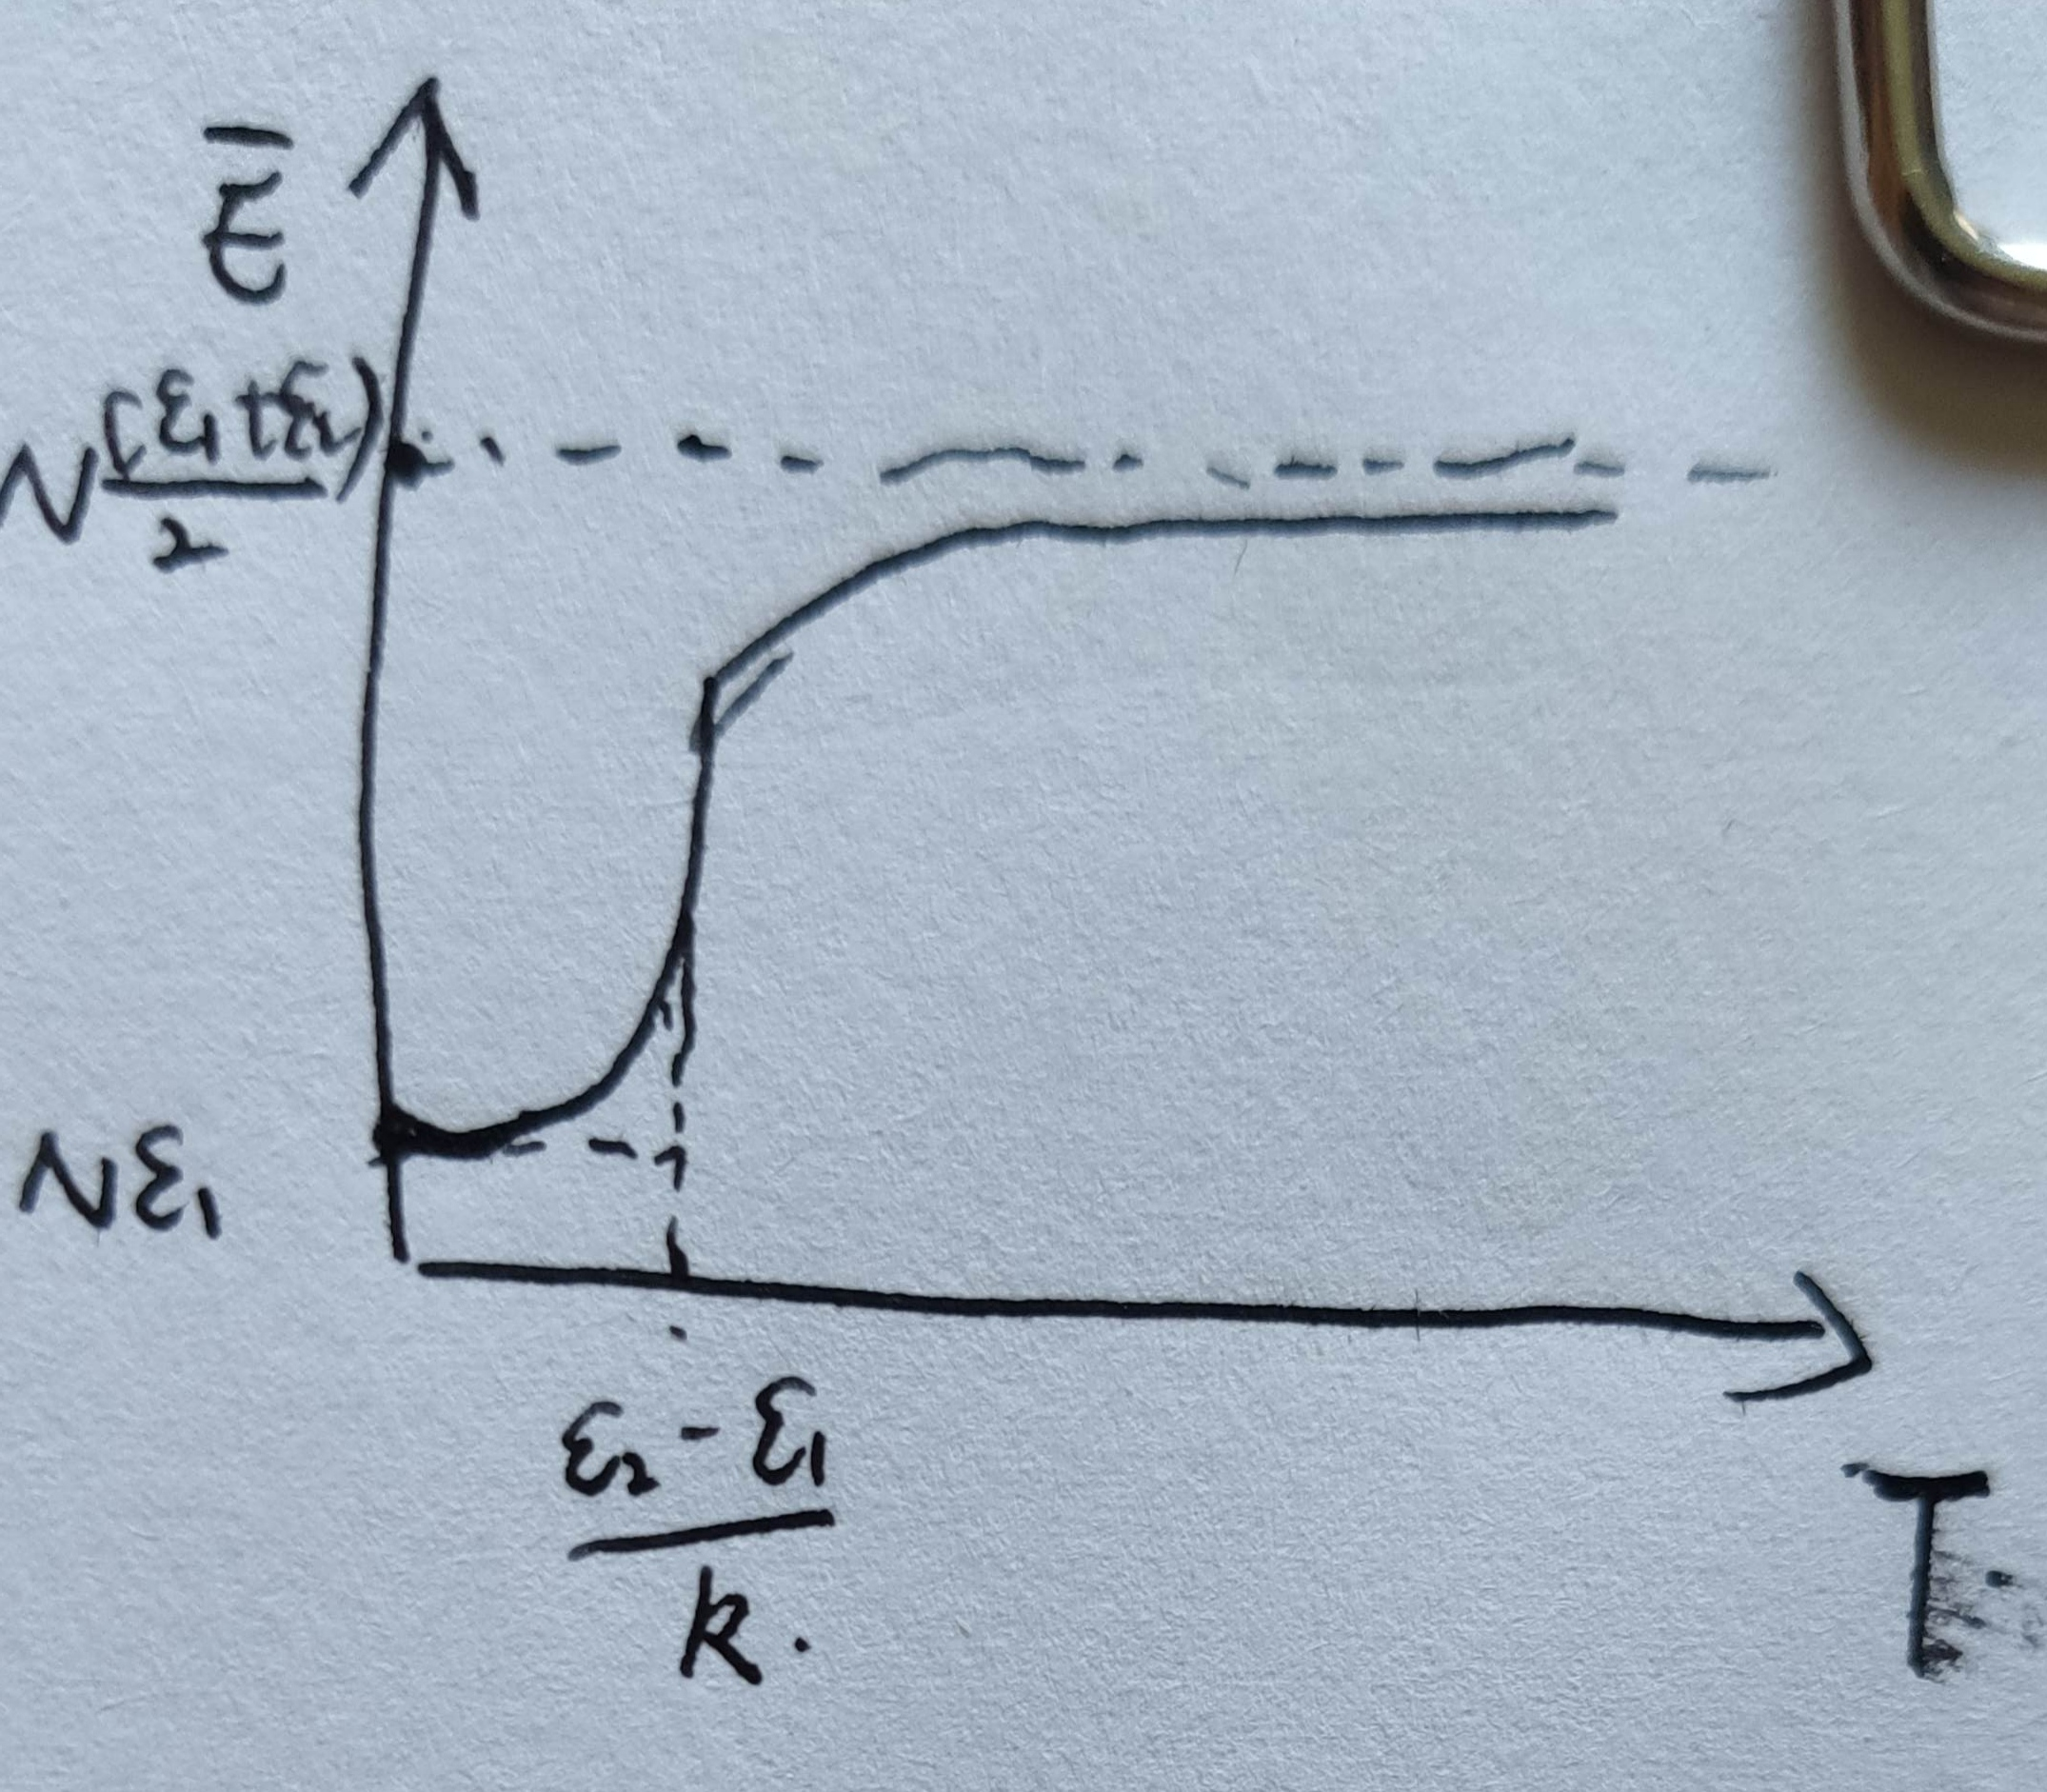
\includegraphics[width = 5.5cm,height = 4cm]{6.6Fig1.jpg}
            \caption{(a)}
        \end{minipage}
        \begin{minipage}[t]{0.45\linewidth}  
            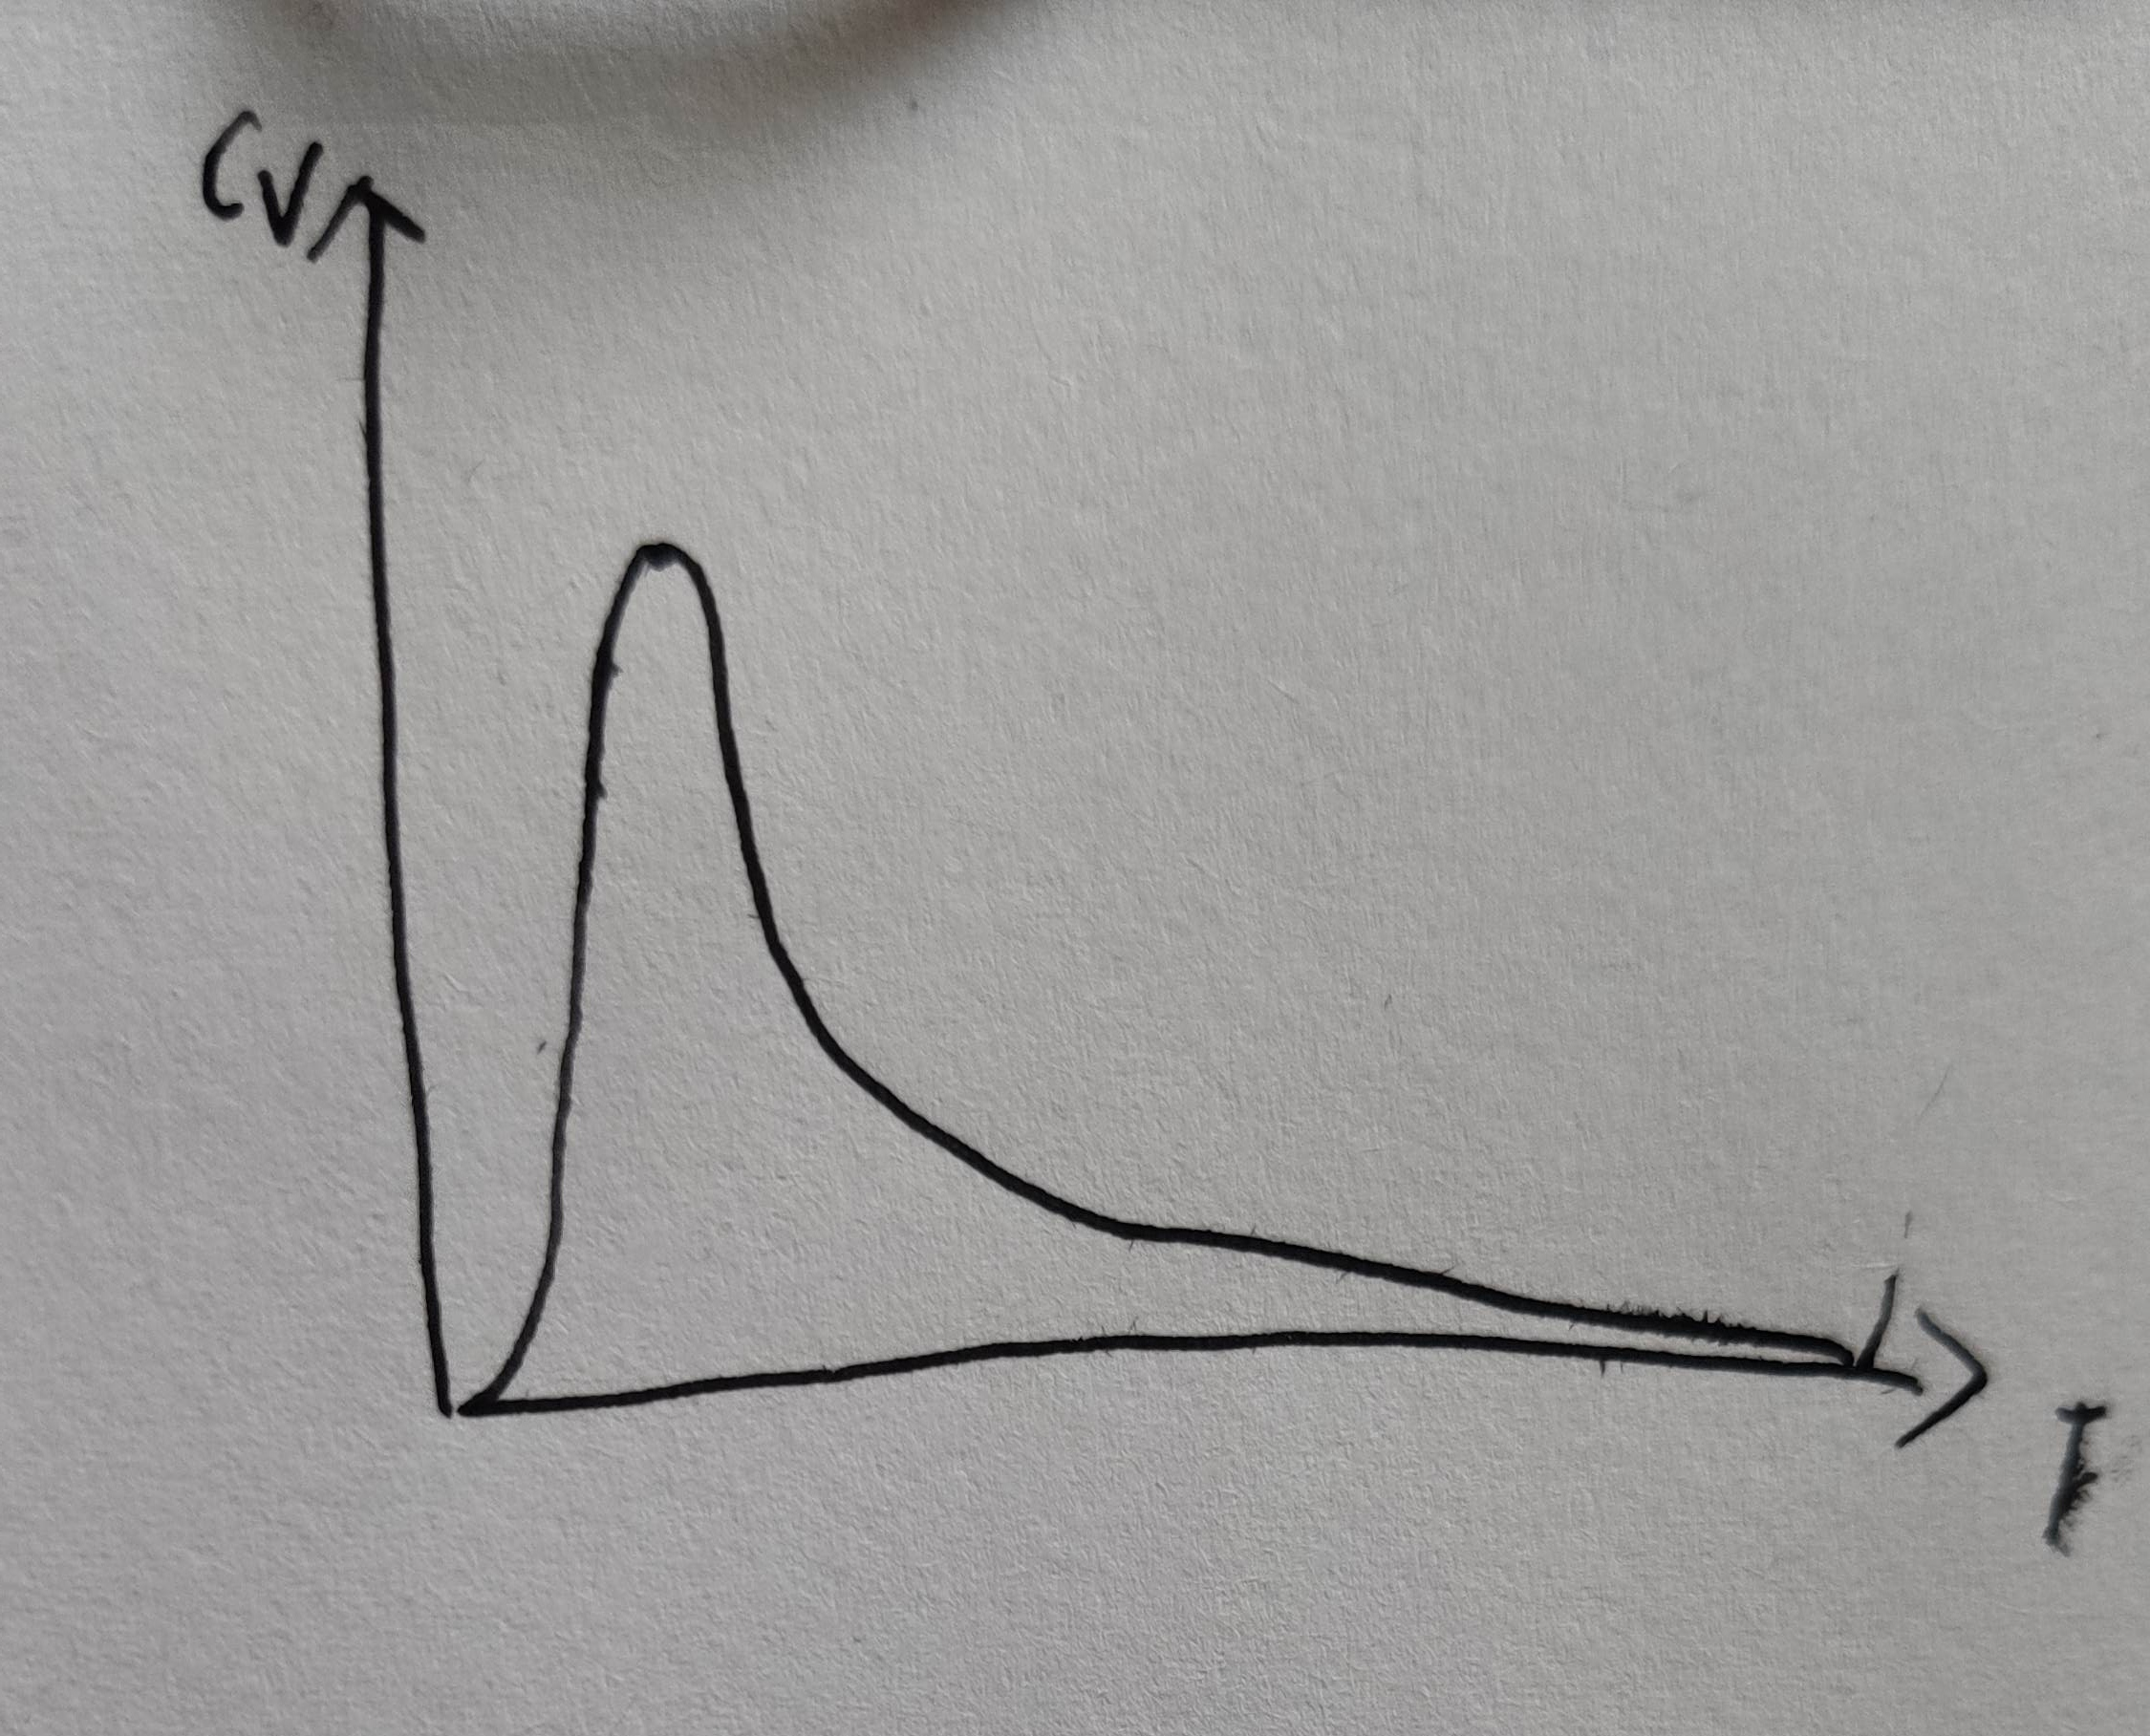
\includegraphics[width = 5.5cm,height = 4cm]{6.6Fig2.jpg}
            \caption{(b)}
        \end{minipage}
    \end{figure}
    As T approaches 0 the system tends to the low energy state, while in the limit of high temperatures all states become equally probable. The energy goes from the low to the high temperature Iimit when $\epsilon_{2}-\epsilon_{1} \approx KT$\\
    The specific heat is, $C_{V}=\left(\frac{\partial \bar{E}}{\partial T}\right)_{V}$, i.e., the slope of $\overline{E}$\\
    (c)\\
    $$\bar{E} = N\left[\frac{\epsilon_1 e^{-\epsilon_1/kT} + \epsilon_2 e^{-\epsilon_2/kT}}{e^{-\epsilon_1/kT}+e^{-\epsilon_2 / kT}}\right] = N\left[\frac{\epsilon_{1}+\epsilon_{2} e^{-\left(\epsilon_{2}-\epsilon_{1}\right) / K T}}{1+e^{-\left(\epsilon_{2}-\epsilon_{1}\right) / K T}}\right] \eqno(5.1)$$
    $$T \to 0,\bar{E} \to N \epsilon_1 \eqno(5.2)$$
    $$T \to \infty, \bar{E} \to N(\frac{\epsilon_1 + \epsilon_2}{2}) \eqno(5.3)$$
    So:
    $$\frac{\epsilon_{2}-\epsilon_{1}}{\mathrm{k} T}=\ln 3 \approx 1 \quad \text { or } \quad\left(\epsilon_{2}-\epsilon_{1}\right) \approx \mathrm{k}T \eqno(5.4)$$
    Then the heat capacity is:
    $$c_{V}=\frac{\partial \bar{E}}{\partial T}=\frac{N\left(\epsilon_{2}-\varepsilon_{1}\right)^{2} e^{-\left(\varepsilon_{2}-\epsilon_{1}\right) / K^{2}}}{K T^{2}\left[1+e^{\left.-\left(\epsilon_{2}-\varepsilon_{1}\right) / K T\right.}\right]^{2}} \eqno(5.5)$$
    $C_V \to 0$ as $T \to 0, T \to \infty$.\\


    Problem 6.10\\
    Answer:\\
    (a)\\
    The centrifugal force $m \omega^2 r$ yields the potential energy $-\frac{m \omega^2 r^2}{2}$. Since the probablilty that a molecule is at r is proportional to the Boltzman factor, the density is:
    $$p(r)=p(0) e^{ m \omega^{2} r^{2} / 2 k T} \eqno(6.1)$$
    (b)\\
    Substituting $\mu_ = N_A m$, the molecular weight, into (6.1) and evaluating this expression at $r_1$ and $r_2$ we have:
    $$\mu=\frac{2 \mathrm{N}_{\mathrm{A}} \mathrm{kT}}{\omega^{2}\left(\mathrm{r}_{1}^{2}-\mathrm{r}_{2}\right)^{2}} \ln \frac{\rho\left(\mathrm{r}_{1}\right)}{\rho\left(\mathrm{r}_{2}\right)} \eqno(6.2)$$

\end{document}
